\documentclass[11pt]{article}
\usepackage[margin=0.9in]{geometry}
\usepackage{amsmath,amssymb}
\usepackage{tikz}
\usetikzlibrary{arrows.meta}
\usepackage{newtxtext,newtxmath}
\setlength{\parskip}{0.5em}
\setlength{\parindent}{0pt}
\sloppy

\tikzset{
  wire/.style={thick},
  cut/.style={densely dashed,red!70!black},
  every node/.style={font=\small},
}
% box from (x1,y1) to (x2,y2) with label
\newcommand{\obox}[5]{\draw[thick,rounded corners=2pt,fill=black!8] (#1,#2) rectangle (#3,#4);\node at ({(#1+#3)/2},{(#2+#4)/2}) {#5};}
\newcommand{\kk}[1]{|#1\rangle\!\rangle}
\newcommand{\bb}[1]{\langle\!\langle #1|}

\begin{document}
\begin{center}
{\large\bfseries Process matrices in pictures (operator convention)}\\[3pt]
{\small Every box is an operator. Its bra indices are wires entering from below, its ket indices
are wires leaving above. Placing one box above another and joining wires is operator multiplication;
a wire looped from the top of a diagram back to its bottom is a trace. A bare vertical wire is the
identity. A dashed red line is a horizontal cut: the rank of what is drawn is at most the product of
the dimensions of the wires the cut crosses.}
\end{center}

\subsection*{1. A state is an operator: the ordinary Born rule}
\begin{center}
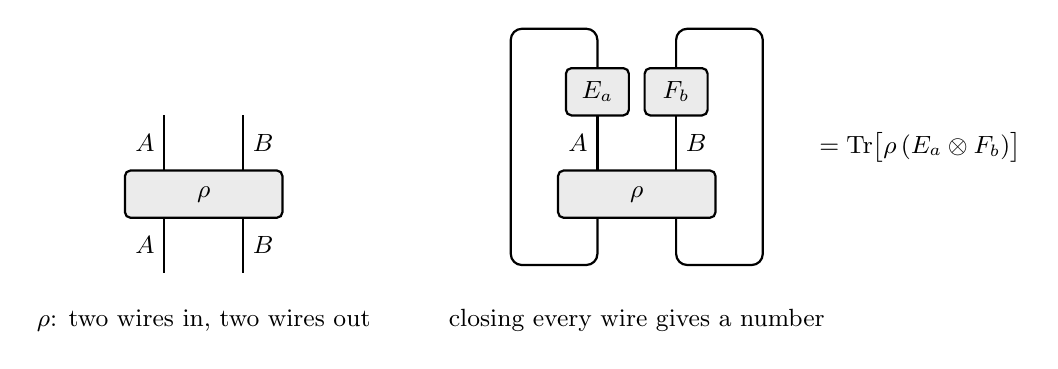
\begin{tikzpicture}[x=1cm,y=1cm]
% rho alone
\obox{-1.0}{-0.3}{1.0}{0.3}{$\rho$}
\draw[wire] (-0.5,-1.0) -- (-0.5,-0.3); \draw[wire] (0.5,-1.0) -- (0.5,-0.3);
\draw[wire] (-0.5,0.3) -- (-0.5,1.0);   \draw[wire] (0.5,0.3) -- (0.5,1.0);
\node[left] at (-0.5,-0.65) {$A$}; \node[right] at (0.5,-0.65) {$B$};
\node[left] at (-0.5,0.65) {$A$};  \node[right] at (0.5,0.65) {$B$};
\node at (0,-1.6) {$\rho$: two wires in, two wires out};
% Born rule
\begin{scope}[xshift=5.5cm]
\obox{-1.0}{-0.3}{1.0}{0.3}{$\rho$}
\draw[wire] (-0.5,0.3) -- (-0.5,1.0); \draw[wire] (0.5,0.3) -- (0.5,1.0);
\obox{-0.9}{1.0}{-0.1}{1.6}{$E_a$} \obox{0.1}{1.0}{0.9}{1.6}{$F_b$}
\draw[wire,rounded corners=4pt] (-0.5,1.6) -- (-0.5,2.1) -- (-1.6,2.1) -- (-1.6,-0.9) -- (-0.5,-0.9) -- (-0.5,-0.3);
\draw[wire,rounded corners=4pt] (0.5,1.6) -- (0.5,2.1) -- (1.6,2.1) -- (1.6,-0.9) -- (0.5,-0.9) -- (0.5,-0.3);
\node[left] at (-0.5,0.65) {$A$}; \node[right] at (0.5,0.65) {$B$};
\node at (3.6,0.6) {$=\operatorname{Tr}\bigl[\rho\,(E_a\otimes F_b)\bigr]$};
\node at (0,-1.6) {closing every wire gives a number};
\end{scope}
\end{tikzpicture}
\end{center}

\subsection*{2. The process matrix $W$ and its Born rule}
\begin{center}
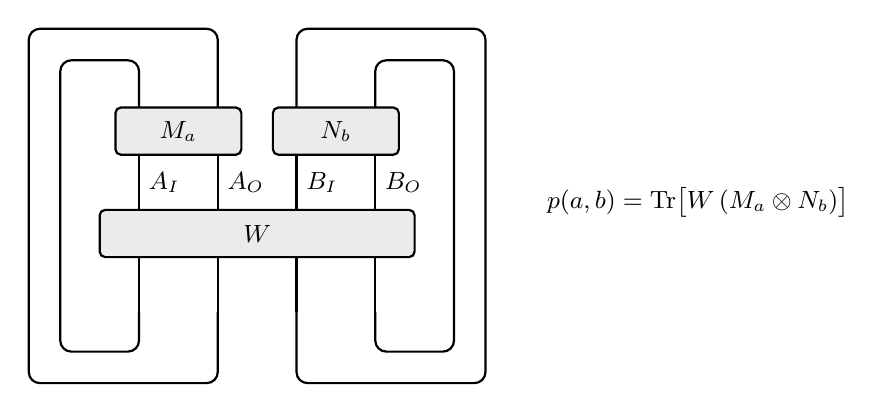
\begin{tikzpicture}[x=1cm,y=1cm]
% W: operator on four wires
\obox{-2.0}{-0.3}{2.0}{0.3}{$W$}
\foreach \x/\l in {-1.5/A_I,-0.5/A_O,0.5/B_I,1.5/B_O} {
  \draw[wire] (\x,0.3) -- (\x,1.0); \draw[wire] (\x,-0.3) -- (\x,-1.0);
  \node[right] at (\x,0.65) {$\l$};
}
\obox{-1.8}{1.0}{-0.2}{1.6}{$M_a$} \obox{0.2}{1.0}{1.8}{1.6}{$N_b$}
% loops: inner leg gets outer loop
\draw[wire,rounded corners=4pt] (-1.5,1.6) -- (-1.5,2.2) -- (-2.5,2.2) -- (-2.5,-1.5) -- (-1.5,-1.5) -- (-1.5,-1.0);
\draw[wire,rounded corners=4pt] (-0.5,1.6) -- (-0.5,2.6) -- (-2.9,2.6) -- (-2.9,-1.9) -- (-0.5,-1.9) -- (-0.5,-1.0);
\draw[wire,rounded corners=4pt] (1.5,1.6) -- (1.5,2.2) -- (2.5,2.2) -- (2.5,-1.5) -- (1.5,-1.5) -- (1.5,-1.0);
\draw[wire,rounded corners=4pt] (0.5,1.6) -- (0.5,2.6) -- (2.9,2.6) -- (2.9,-1.9) -- (0.5,-1.9) -- (0.5,-1.0);
\node at (5.6,0.4) {$p(a,b)=\operatorname{Tr}\bigl[W\,(M_a\otimes N_b)\bigr]$};
\end{tikzpicture}
\end{center}
Alice's instrument element is a CP map $A_I\to A_O$, but we never draw the map: we draw its Choi
matrix $M_a$, an operator on $A_I\otimes A_O$, so a box with two wires in and two wires out, exactly
like $\rho$ in picture~1. Likewise $N_b$. The process matrix $W$ is an operator on all four wires.
The Born rule is the same closed diagram as in picture~1 with $\rho\to W$ and $E_a,F_b\to M_a,N_b$.
Validity of $W$: the closed diagram equals $1$ whenever $M_a,N_b$ are summed over outcomes. There is
no separate $\rho$ in this formalism; $W$ is the only state-like object, and any state handed to the
laboratories is part of $W$ (next picture).

\subsection*{3. Two familiar $W$'s, drawn as operators}
\begin{center}
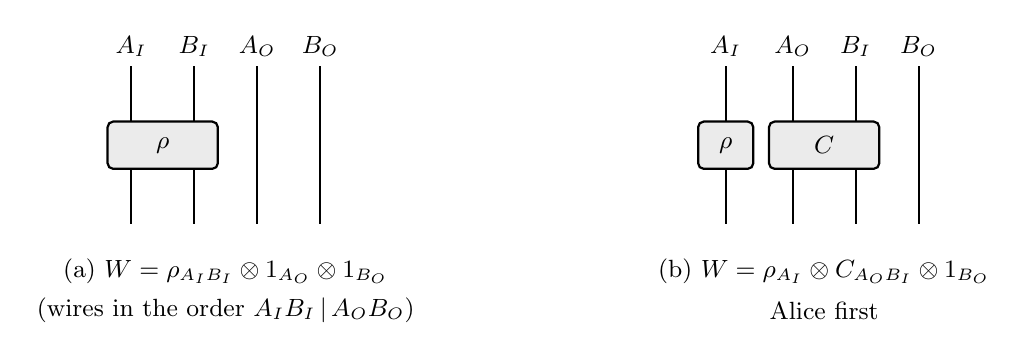
\begin{tikzpicture}[x=1cm,y=1cm]
% (a) rho tensor 1 tensor 1, wires reordered A_I B_I | A_O B_O
\begin{scope}
\obox{-1.5}{-0.3}{-0.1}{0.3}{$\rho$}
\foreach \x/\l in {-1.2/A_I,-0.4/B_I} {\draw[wire] (\x,0.3)--(\x,1.0); \draw[wire] (\x,-0.3)--(\x,-1.0); \node[above] at (\x,1.0) {$\l$};}
\foreach \x/\l in {0.4/A_O,1.2/B_O} {\draw[wire] (\x,-1.0)--(\x,1.0); \node[above] at (\x,1.0) {$\l$};}
\node at (0,-1.6) {(a) $W=\rho_{A_IB_I}\otimes 1_{A_O}\otimes 1_{B_O}$};
\node at (0,-2.1) {(wires in the order $A_IB_I\,|\,A_OB_O$)};
\end{scope}
% (b) rho tensor C tensor 1
\begin{scope}[xshift=7.6cm]
\obox{-1.6}{-0.3}{-0.9}{0.3}{$\rho$}
\obox{-0.7}{-0.3}{0.7}{0.3}{$C$}
\foreach \x/\l in {-1.25/A_I,-0.4/A_O,0.4/B_I} {\draw[wire] (\x,0.3)--(\x,1.0); \draw[wire] (\x,-0.3)--(\x,-1.0); \node[above] at (\x,1.0) {$\l$};}
\draw[wire] (1.2,-1.0)--(1.2,1.0); \node[above] at (1.2,1.0) {$B_O$};
\node at (0,-1.6) {(b) $W=\rho_{A_I}\otimes C_{A_OB_I}\otimes 1_{B_O}$};
\node at (0,-2.1) {Alice first};
\end{scope}
\end{tikzpicture}
\end{center}
In (a), contracting with $M_a\otimes N_b$ as in picture~2, the bare wires $A_O,B_O$ just trace
$M_a$ and $N_b$ over their output index, leaving POVM elements on $A_I,B_I$, and one recovers
picture~1. In (b), $C$ is the Choi matrix of a channel: the box sits on the pair ($A_O$, $B_I$)
because it connects Alice's output to Bob's input. A causally separable $W$ is a convex combination of
(b) and its mirror image. The content of the subject is that there are valid $W$'s of neither form.

\subsection*{4. The Choi isomorphism, and what ``rank one'' looks like}
\begin{center}
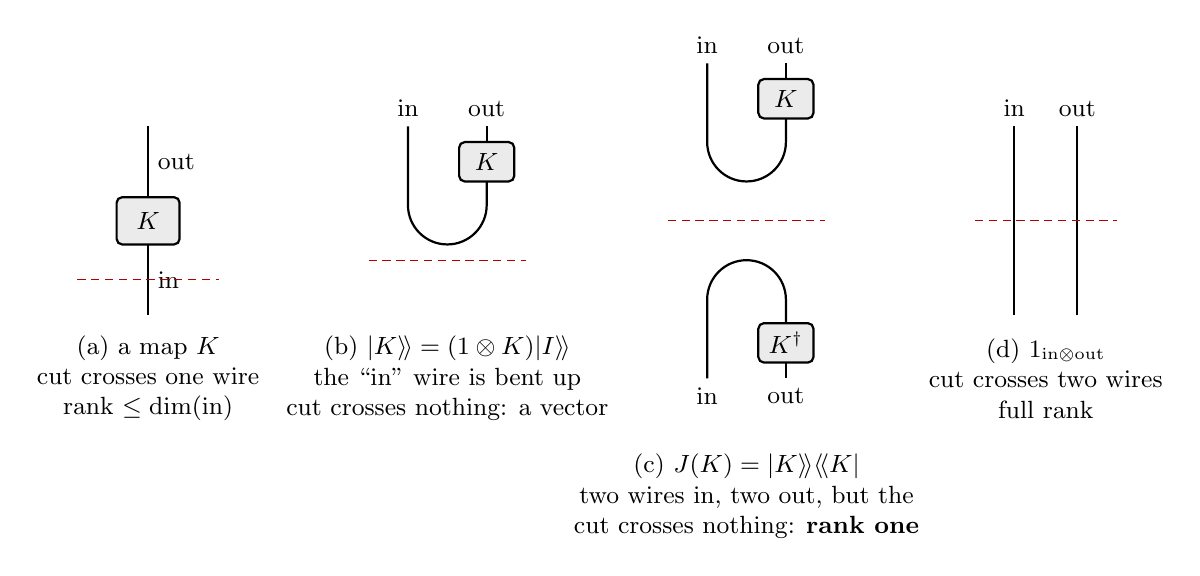
\begin{tikzpicture}[x=1cm,y=1cm]
% (a) K as a map
\begin{scope}
\obox{-0.4}{-0.3}{0.4}{0.3}{$K$}
\draw[wire] (0,-0.3)--(0,-1.2); \draw[wire] (0,0.3)--(0,1.2);
\node[right] at (0,-0.75) {in}; \node[right] at (0,0.75) {out};
\draw[cut] (-0.9,-0.75)--(0.9,-0.75);
\node[align=center] at (0,-2.0) {(a) a map $K$\\ cut crosses one wire\\ rank $\le\dim(\text{in})$};
\end{scope}
% (b) vector
\begin{scope}[xshift=3.8cm]
\draw[wire] (-0.5,1.2) -- (-0.5,0.2) arc (180:360:0.5) -- (0.5,0.5);
\obox{0.15}{0.5}{0.85}{1.0}{$K$}
\draw[wire] (0.5,1.0)--(0.5,1.2);
\node[above] at (-0.5,1.2) {in}; \node[above] at (0.5,1.2) {out};
\draw[cut] (-1.0,-0.5)--(1.0,-0.5);
\node[align=center] at (0,-2.0) {(b) $\kk{K}=(1\otimes K)\kk{I}$\\ the ``in'' wire is bent up\\ cut crosses nothing: a vector};
\end{scope}
% (c) projector
\begin{scope}[xshift=7.6cm]
\draw[wire] (-0.5,2.0) -- (-0.5,1.0) arc (180:360:0.5) -- (0.5,1.3);
\obox{0.15}{1.3}{0.85}{1.8}{$K$}
\draw[wire] (0.5,1.8)--(0.5,2.0);
\draw[wire] (-0.5,-2.0) -- (-0.5,-1.0) arc (180:0:0.5) -- (0.5,-1.3);
\obox{0.15}{-1.8}{0.85}{-1.3}{$K^\dagger$}
\draw[wire] (0.5,-1.8)--(0.5,-2.0);
\node[above] at (-0.5,2.0) {in}; \node[above] at (0.5,2.0) {out};
\node[below] at (-0.5,-2.0) {in}; \node[below] at (0.5,-2.0) {out};
\draw[cut] (-1.0,0)--(1.0,0);
\node[align=center] at (0,-3.5) {(c) $J(K)=\kk{K}\bb{K}$\\ two wires in, two out, but the\\ cut crosses nothing: \textbf{rank one}};
\end{scope}
% (d) identity on in x out
\begin{scope}[xshift=11.4cm]
\draw[wire] (-0.4,-1.2)--(-0.4,1.2); \draw[wire] (0.4,-1.2)--(0.4,1.2);
\node[above] at (-0.4,1.2) {in}; \node[above] at (0.4,1.2) {out};
\draw[cut] (-0.9,0)--(0.9,0);
\node[align=center] at (0,-2.0) {(d) $1_{\text{in}\otimes\text{out}}$\\ cut crosses two wires\\ full rank};
\end{scope}
\end{tikzpicture}
\end{center}
The map $K$ in (a) is a matrix with rows ``out'' and columns ``in''; if it is unitary it is full
rank, and the cut below it crosses its ``in'' wire. Bending that wire upward with the identity state
$\kk{I}=\sum_k|k\rangle|k\rangle$ gives the vector (b): the \emph{same numbers} $K_{mn}$, now
indexing a single vector on in$\,\otimes\,$out. The Choi matrix (c) is that vector times its dual.
As an operator on in$\,\otimes\,$out it has two wires in and two out, like (d), but between the ket
half and the bra half there is a gap that no wire crosses: that is what rank one means. Nothing about
unitarity was used; (c) is rank one for any $K$.

\subsection*{5. Where $\rho$ enters, and why $K^\dagger K=1$}
\begin{center}
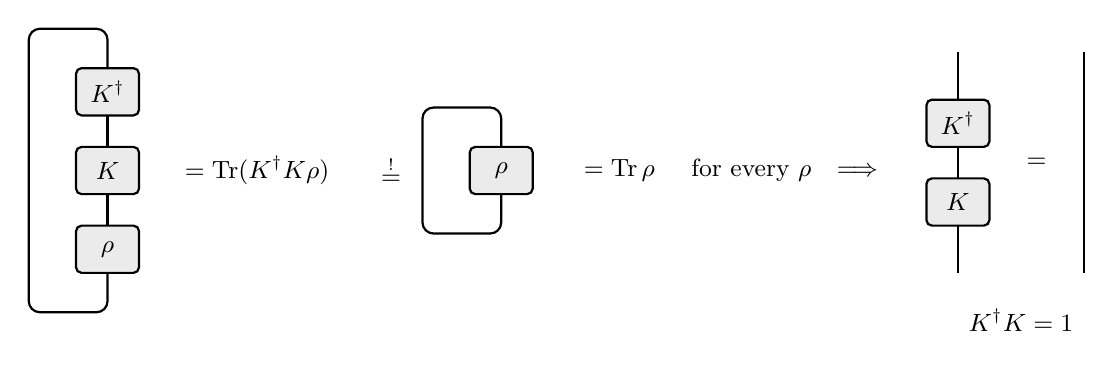
\begin{tikzpicture}[x=1cm,y=1cm]
% Tr(K^dag K rho)
\obox{-0.4}{-0.3}{0.4}{0.3}{$\rho$}
\obox{-0.4}{0.7}{0.4}{1.3}{$K$}
\obox{-0.4}{1.7}{0.4}{2.3}{$K^\dagger$}
\draw[wire] (0,0.3)--(0,0.7); \draw[wire] (0,1.3)--(0,1.7);
\draw[wire,rounded corners=4pt] (0,2.3)--(0,2.8)--(-1.0,2.8)--(-1.0,-0.8)--(0,-0.8)--(0,-0.3);
\node at (1.9,1.0) {$=\operatorname{Tr}(K^\dagger K\rho)$};
\node at (3.6,1.0) {$\overset{!}{=}$};
\begin{scope}[xshift=5.0cm]
\obox{-0.4}{0.7}{0.4}{1.3}{$\rho$}
\draw[wire,rounded corners=4pt] (0,1.3)--(0,1.8)--(-1.0,1.8)--(-1.0,0.2)--(0,0.2)--(0,0.7);
\node at (1.5,1.0) {$=\operatorname{Tr}\rho$};
\end{scope}
\node at (8.6,1.0) {for every $\rho$\quad$\Longrightarrow$};
\begin{scope}[xshift=10.8cm]
\obox{-0.4}{0.3}{0.4}{0.9}{$K$}
\obox{-0.4}{1.3}{0.4}{1.9}{$K^\dagger$}
\draw[wire] (0,-0.3)--(0,0.3); \draw[wire] (0,0.9)--(0,1.3); \draw[wire] (0,1.9)--(0,2.5);
\node at (1.0,1.1) {$=$};
\draw[wire] (1.6,-0.3)--(1.6,2.5);
\node at (0.8,-0.9) {$K^\dagger K=1$};
\end{scope}
\end{tikzpicture}
\end{center}
Multiplying $\rho$ by $K$ and then $K^\dagger$ and closing the wire is $\operatorname{Tr}(K^\dagger K\rho)$.
Trace preservation of $\rho\mapsto K\rho K^\dagger$ demands that this equal $\operatorname{Tr}\rho$ for
\emph{every} $\rho$. The state is a separate box plugged into the open wire; it is not inside $K$. Since
the equality holds for all $\rho$, the box $\rho$ can be removed from the statement, leaving the operator
identity $K^\dagger K=1$ on the right. This uses only normalization; unitarity would add $KK^\dagger=1$,
i.e.\ $K$ square and invertible.

\subsection*{6. A pure process, and the swap argument}
\begin{center}
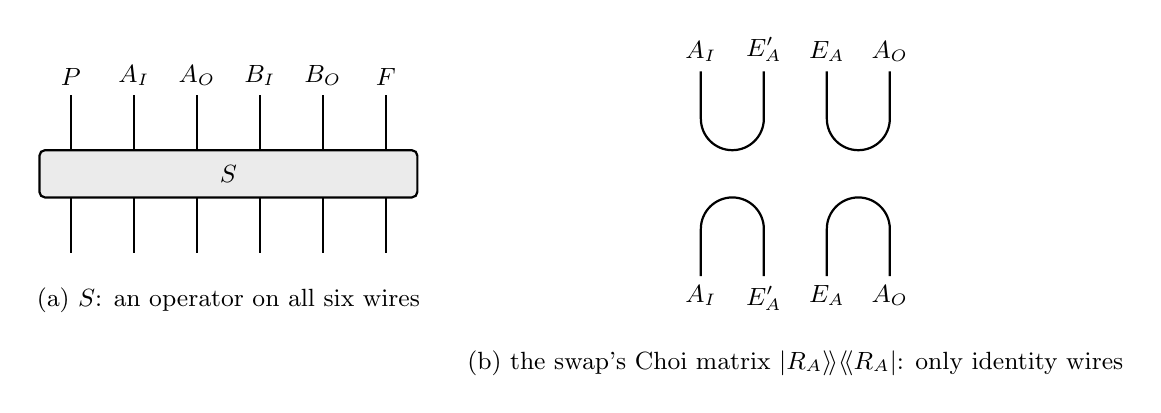
\begin{tikzpicture}[x=1cm,y=1cm]
% (a) S as operator on six wires
\begin{scope}
\obox{-2.4}{-0.3}{2.4}{0.3}{$S$}
\foreach \x/\l in {-2.0/P,-1.2/A_I,-0.4/A_O,0.4/B_I,1.2/B_O,2.0/F} {
  \draw[wire] (\x,0.3)--(\x,1.0); \draw[wire] (\x,-0.3)--(\x,-1.0); \node[above] at (\x,1.0) {$\l$};}
\node at (0,-1.6) {(a) $S$: an operator on all six wires};
\end{scope}
% (b) the swap's Choi matrix: two cups over two caps
\begin{scope}[xshift=7.2cm]
\draw[wire] (-1.2,1.3) -- (-1.2,0.7) arc (180:360:0.4) -- (-0.4,1.3);
\draw[wire] (0.4,1.3) -- (0.4,0.7) arc (180:360:0.4) -- (1.2,1.3);
\draw[wire] (-1.2,-1.3) -- (-1.2,-0.7) arc (180:0:0.4) -- (-0.4,-1.3);
\draw[wire] (0.4,-1.3) -- (0.4,-0.7) arc (180:0:0.4) -- (1.2,-1.3);
\foreach \x/\l in {-1.2/A_I,-0.4/E'_A,0.4/E_A,1.2/A_O} {\node[above] at (\x,1.3) {$\l$}; \node[below] at (\x,-1.3) {$\l$};}
\node at (0,-2.4) {(b) the swap's Choi matrix $\kk{R_A}\bb{R_A}$: only identity wires};
\end{scope}
\end{tikzpicture}

\vspace{4pt}
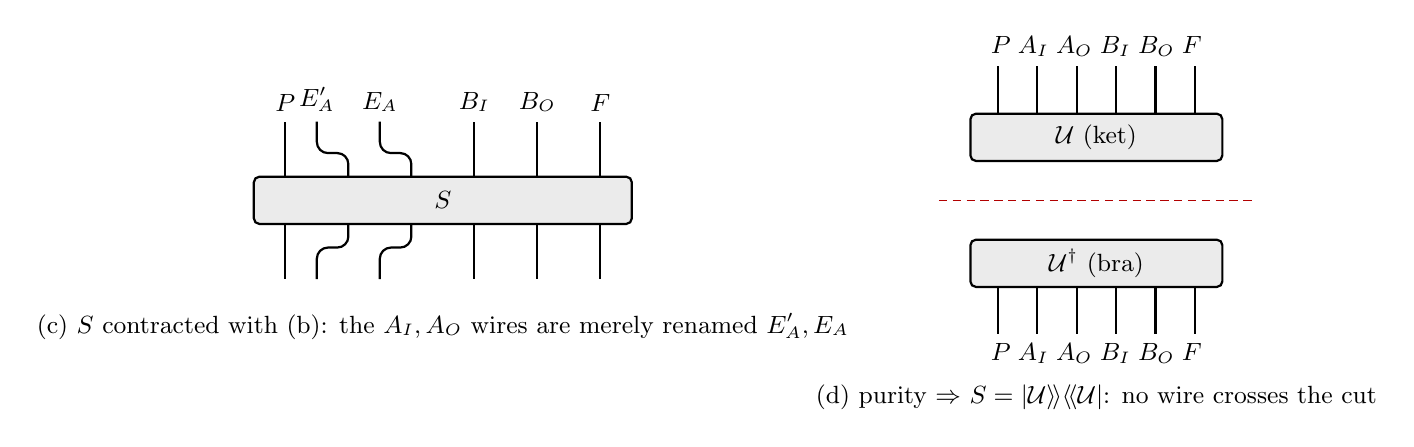
\begin{tikzpicture}[x=1cm,y=1cm]
% (c) contraction = renaming
\begin{scope}
\obox{-2.4}{-0.3}{2.4}{0.3}{$S$}
\foreach \x/\l in {-2.0/P,0.4/B_I,1.2/B_O,2.0/F} {
  \draw[wire] (\x,0.3)--(\x,1.0); \draw[wire] (\x,-0.3)--(\x,-1.0); \node[above] at (\x,1.0) {$\l$};}
% A_I wire bent via cup to E'_A position; A_O wire via cup to E_A position (drawn as rerouted wires)
\draw[wire,rounded corners=4pt] (-1.2,0.3)--(-1.2,0.6)--(-1.6,0.6)--(-1.6,1.0);
\draw[wire,rounded corners=4pt] (-1.2,-0.3)--(-1.2,-0.6)--(-1.6,-0.6)--(-1.6,-1.0);
\draw[wire,rounded corners=4pt] (-0.4,0.3)--(-0.4,0.6)--(-0.8,0.6)--(-0.8,1.0);
\draw[wire,rounded corners=4pt] (-0.4,-0.3)--(-0.4,-0.6)--(-0.8,-0.6)--(-0.8,-1.0);
\node[above] at (-1.6,1.0) {$E'_A$}; \node[above] at (-0.8,1.0) {$E_A$};
\node at (0,-1.6) {(c) $S$ contracted with (b): the $A_I,A_O$ wires are merely renamed $E'_A,E_A$};
\end{scope}
% (d) purity => rank one
\begin{scope}[xshift=8.3cm]
\obox{-1.6}{0.5}{1.6}{1.1}{$\mathcal U$ (ket)}
\obox{-1.6}{-1.1}{1.6}{-0.5}{$\mathcal U^\dagger$ (bra)}
\foreach \x in {-1.25,-0.75,-0.25,0.25,0.75,1.25} {\draw[wire] (\x,1.1)--(\x,1.7); \draw[wire] (\x,-1.1)--(\x,-1.7);}
\node[above] at (0,1.7) {$P\;A_I\;A_O\;B_I\;B_O\;F$};
\node[below] at (0,-1.7) {$P\;A_I\;A_O\;B_I\;B_O\;F$};
\draw[cut] (-2.0,0)--(2.0,0);
\node at (0,-2.5) {(d) purity $\Rightarrow$ $S=\kk{\mathcal U}\bb{\mathcal U}$: no wire crosses the cut};
\end{scope}
\end{tikzpicture}
\end{center}
(a) A process with past and future is an operator on six wires. Its Born rule contracts $P$ with a
past state, the four laboratory wires with $M_a\otimes N_b$, and $F$ with a measurement on the future.
(b) The local operation ``swap $A_I$ out to $E'_A$, $E_A$ in to $A_O$'' has a Choi matrix made of
nothing but identity wires. (c) Contracting $S$ with it therefore does nothing except carry the $A_I$
wires to the $E'_A$ position and the $A_O$ wires to the $E_A$ position: the result is $S$ itself, now
read as an operator with wires $P,E_A,E_B$ and $F,E'_A,E'_B$, i.e.\ as the Choi matrix of a map
$\mathcal U\colon P\otimes A_O\otimes B_O\to A_I\otimes B_I\otimes F$. Purity says this map is a unitary.
Picture~4 then says that $S$ is a ket over a bra with nothing between them, (d). Picture~5, with the
``every $\rho$'' running over states of $P\otimes E_A\otimes E_B$, says $\mathcal U^\dagger\mathcal U=1$.

\subsection*{7. From $S$ back to $W$: plugging in $|0\rangle$ and tracing out $F$}
\begin{center}
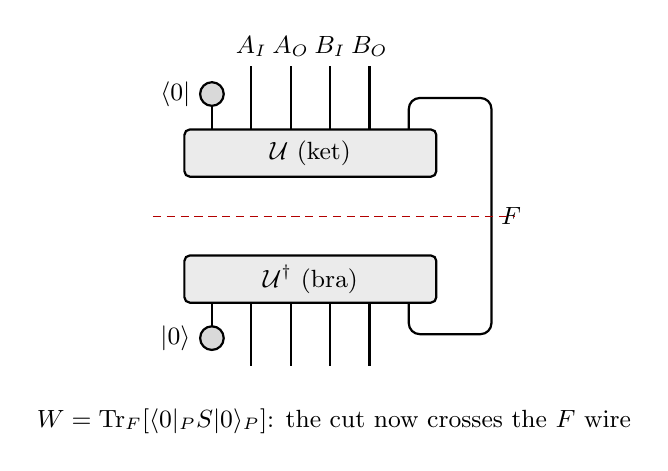
\begin{tikzpicture}[x=1cm,y=1cm]
\obox{-1.6}{0.5}{1.6}{1.1}{$\mathcal U$ (ket)}
\obox{-1.6}{-1.1}{1.6}{-0.5}{$\mathcal U^\dagger$ (bra)}
\foreach \x/\l in {-0.75/A_I,-0.25/A_O,0.25/B_I,0.75/B_O} {\draw[wire] (\x,1.1)--(\x,1.9); \draw[wire] (\x,-1.1)--(\x,-1.9); \node[above] at (\x,1.9) {$\l$};}
% P: plug |0> below ket (ket's P wire is an out wire; W = <0|S|0>: contract S's P-out with <0| and P-in with |0>)
\draw[wire] (-1.25,1.1)--(-1.25,1.4); \draw[thick,fill=black!15] (-1.25,1.55) circle (0.15); \node[left] at (-1.4,1.55) {$\langle0|$};
\draw[wire] (-1.25,-1.1)--(-1.25,-1.4); \draw[thick,fill=black!15] (-1.25,-1.55) circle (0.15); \node[left] at (-1.4,-1.55) {$|0\rangle$};
% F: trace loop connecting ket's F wire to bra's F wire
\draw[wire,rounded corners=4pt] (1.25,1.1)--(1.25,1.5)--(2.3,1.5)--(2.3,-1.5)--(1.25,-1.5)--(1.25,-1.1);
\node[right] at (2.3,0) {$F$};
\draw[cut] (-2.0,0)--(2.6,0);
\node at (0.3,-2.6) {$W=\operatorname{Tr}_F[\langle0|_P S|0\rangle_P]$: the cut now crosses the $F$ wire};
\end{tikzpicture}
\end{center}
$S$ contains no state on $P$; the state is supplied from outside, as the two dots $\langle0|$ and
$|0\rangle$ attached to the open $P$ wires (one on the ket side, one on the bra side, because
$W=\langle0|S|0\rangle$ contracts both). Discarding $F$ is a wire looped from the ket's $F$ to the bra's
$F$. What is left has only the four laboratory wires open: it is a bipartite process matrix $W$ as in
picture~2. And the horizontal cut that crossed nothing in picture~6(d) now crosses the $F$ loop, so
$W$ can have rank up to $\dim F$. This is how a rank-one $S$ produces a mixed $W$, and it is the step
in the purification theorem where coherence between causal orders is lost.
\end{document}
